%\documentclass[openany]{book}
\documentclass[12pt]{article}
\usepackage[utf8]{inputenc}
\usepackage{amssymb} %for fancy L
\usepackage{calrsfs} %for fancy L
\usepackage{cancel}
\usepackage{tabularx}
\usepackage[hyphens]{url}
\usepackage{booktabs}
\usepackage{graphicx}
\usepackage[titletoc,title]{appendix}
\usepackage{subfig}
\DeclareMathAlphabet{\pazocal}{OMS}{zplm}{m}{n} %for fancy L
\usepackage{epsfig, float,array,tabu,longtable,}
\usepackage{hyperref,wrapfig}
\usepackage{enumerate}
\usepackage{graphicx,psfrag}
\usepackage{cite}
\usepackage{sectsty}
\usepackage{epstopdf}
\usepackage{amsmath,esint, setspace, fancyhdr, amsfonts, bookmark, blindtext}
\usepackage[normalem]{ulem}
\usepackage{tikz}
\usepackage{rotating}
\usepackage[americanvoltages,fulldiodes,siunitx]{circuitikz}
\usepackage{stackengine}
\usetikzlibrary{matrix}
\usepackage{multirow}
\usepackage{multicol}
\usetikzlibrary{shapes,backgrounds,patterns}
\usetikzlibrary{mindmap,trees,decorations.markings}
\usetikzlibrary{quotes,angles}
\usepackage{verbatim}
\renewcommand{\baselinestretch}{1}
\setlength{\textheight}{8in}
\setlength{\textwidth}{6.5in}
\setlength{\headheight}{0in}
\setlength{\headsep}{0.25in}
\usepackage{graphicx}
\setlength{\topmargin}{0in}
\setlength{\oddsidemargin}{0in}
\setlength{\evensidemargin}{0in}
\setlength{\parindent}{.3in}
\usepackage{listings}
\usepackage{subcaption}
\usepackage{subfig}
\usepackage{tikz}
\usetikzlibrary{decorations}
\usepackage[T1]{fontenc}
%\newcommand\tau{\mathcal{T}}% Caligraphic T for example
\DeclareMathAlphabet{\mathpzc}{OT1}{pzc}{m}{it}
\usepackage{color} %red, green, blue, yellow, cyan, magenta, black, white
\definecolor{mygreen}{RGB}{28,172,0} % color values Red, Green, Blue
\definecolor{mylilas}{RGB}{170,55,241}
% \onehalfspacing
\begin{document}


\begin{titlepage}

 \begin{tikzpicture}[remember picture,overlay,inner sep=0,outer sep=0]
     \draw[black,line width=2pt] ([xshift=-1.5cm,yshift=-2cm]current page.north east) coordinate (A)--([xshift=1.5cm,yshift=-2cm]current page.north west) coordinate(B)--([xshift=1.5cm,yshift=2cm]current page.south west) coordinate (C)--([xshift=-1.5cm,yshift=2cm]current page.south east) coordinate(D)--cycle;

    %  \draw ([yshift=0.5cm,xshift=-0.5cm]A)-- ([yshift=0.5cm,xshift=0.5cm]B)--
    %  ([yshift=-0.5cm,xshift=0.5cm]B) --([yshift=-0.5cm,xshift=-0.5cm]B)--([yshift=0.5cm,xshift=-0.5cm]C)--([yshift=0.5cm,xshift=0.5cm]C)--([yshift=-0.5cm,xshift=0.5cm]C)-- ([yshift=-0.5cm,xshift=-0.5cm]D)--([yshift=0.5cm,xshift=-0.5cm]D)--([yshift=0.5cm,xshift=0.5cm]D)--([yshift=-0.5cm,xshift=0.5cm]A)--([yshift=-0.5cm,xshift=-0.5cm]A)--([yshift=0.5cm,xshift=-0.5cm]A);


     \draw ([yshift=-0.3cm,xshift=0.3cm]A)-- ([yshift=-0.3cm,xshift=-0.3cm]B)--
     ([yshift=0.3cm,xshift=-0.3cm]B) --([yshift=0.3cm,xshift=0.3cm]B)--([yshift=-0.3cm,xshift=0.3cm]C)--([yshift=-0.3cm,xshift=-0.3cm]C)--([yshift=0.3cm,xshift=-0.3cm]C)-- ([yshift=0.3cm,xshift=0.3cm]D)--([yshift=-0.3cm,xshift=0.3cm]D)--([yshift=-0.3cm,xshift=-0.3cm]D)--([yshift=0.3cm,xshift=-0.3cm]A)--([yshift=0.3cm,xshift=0.3cm]A)--([yshift=-0.3cm,xshift=0.3cm]A);

   \end{tikzpicture}

\newcommand{\HRule}{\rule{\linewidth}{0.5mm}} % Defines a new command for the horizontal lines, change thickness here

\center % Center everything on the page
 
%---------------------------------------------------------
%	HEADING SECTIONS
%---------------------------------------------------------


\newcommand*{\plogo}{
\includegraphics[width=0.5\textwidth]{images/wsu}}

\plogo\\[1cm]

\textsc{\large School of Electrical Engineering and Computer Science}\\[1.5cm] % Name of your university/college
 % Major heading such as course name
\textsc{\large \text{Ph.D. Preliminary Examination Report}}\\ % Minor heading such as course title

%---------------------------------------------------------
%	TITLE SECTION
%---------------------------------------------------------

\HRule \\
{ \Large \bfseries Resilience of Power Distribution Networks: \\
\vspace{0.2 cm}
Evaluation and Quantification}\\[0.3cm] % Title of your document
\HRule \\
 
%---------------------------------------------------------
%	AUTHOR SECTION
%---------------------------------------------------------

%\begin{minipage}{0.4\textwidth}

\medskip
\large
{{\textbf{Submitted By}:\\ Shiva Poudel }}\\ [0.5cm]

\medskip

\textbf{Committee Chair}:\\ Dr. Anamika Dubey$^{\dagger}$ \\ [0.5 cm]
\textbf{Committee Members:} \\ Dr. Anjan Bose$^{\dagger}$\\
Dr. Noel N. Schulz$^{\dagger}$\\
Dr. Kevin P. Schneider$^{\S}$\\ 
\vspace{1.5 cm}
\small $^{\dagger}$School of EECS, Washington State University, Pullman, WA, 99164\\
\small $^{\S}$Seattle Research Center, Pacific Northwest National Laboratory, Seattle, WA, 98109\\
\vspace{1.0 cm}
\small
\textbf{Date}: 2/19/2019 \ \ \textbf{Time}: 12:00 PM to 2:00 PM \ \ \textbf{Location}: EME 26 \& via Skype

%---------------------------------------------------------
\setstretch{1.0}

\vfill % Fill the rest of the page with whitespace
\end{titlepage}

\newpage

\textbf{\centering \large Abstract \\}

\vspace{0.9 cm}
 Extreme weather events have a significant impact on the aging and outdated power distribution infrastructures. These high-impact low-probability (HILP) events often result in extended outages and loss of critical services, thus, severely affecting customers' safety. This calls for the need to ensure resilience in distribution networks by quickly restoring the critical services during a disaster. 
 First, the proposal aims to investigate the approaches for resilient restoration of power distribution networks using distributed energy resources (DERs). During an extreme event, locally available DERs are utilized for restoration of critical loads. The proposed framework restores critical loads in the feeder while maximizing the post-restoration reliability of restored loads, including tie switches and open-loop distribution system configurations into the optimization formulation, and optimally allocating DERs for an equitable restoration of the critical loads. 
 Second, we present a new unified decision-making framework that can assist in recovery from both minor and major disruptions in a computationally tractable manner while efficiently utilizing DG resources. The proposed formulation is a unified framework to support both the traditional restoration using feeder reconfiguration and the grid-forming DG-assisted intentional islanding methods. 
 Finally, we propose a probabilistic metric to quantify the operational resilience of the distribution grid. The metric is based on Conditional Value-at-Risk ($CVaR$) measure where resilience is defined as the conditional expectation of loss of energy in MWh for events beyond a pre-specified risk threshold. A simulation-based framework to evaluate the proposed metric for resilience under different weather scenarios is presented. The impacts of smart actions, specifically improved restoration using distributed generators (DGs) and the impacts of infrastructure hardening on resilience metric is also investigated. 

\newpage
\tableofcontents
\newpage




% EXECUTIVE SUMMARY %%%%%%%%%%%%%%%%%%%%%%%%%%%%%%%%%%
\setstretch{1.15}
\section{Motivation}
 The electric power grid is one of the most critical infrastructures of a nation; virtually every aspect of a modern society (transportation, water supply, school, city halls, airports and so on) relies on the supply of electricity. Unfortunately, the increased frequency, duration, and intensity of extreme weather events pose severe threats to the power grid causing wide-area power outages primarily affecting in low- and mid-voltage power distribution grid that contributes to an estimated of 90\% of the outages \cite{farhangi2010path}. This calls for the critical need to improve distribution system resilience for natural disasters. Grid resilience is characterized by its ability to withstand and recover from the high-impact low-probability events \cite{panteli2015grid}. One of the requirements for a resilient distribution system is the ability to restore power to the critical loads for the duration of the outage.
 After extreme natural events, distribution networks may not be able to connect with the bulk power system. Recently, more and more remote-controlled automatic switch facilities are being deployed in the distribution system by utilities via distribution automation programs in order to achieve the vision of a ``self-healing'' grid \cite{program}.  With the help of remotely controlled tie-switches and sectionalizing switches, distributed generators (DGs) can be exploited to restore more loads (instead of just supplying the nearby or local load) by forming a self-sustained islanded grid (SSIG). 
  
  Usually, during an outage caused by extreme events, it takes several days and sometimes even weeks and months to restore the normal power supply. A recent example is an outage in Puerto Rico because of hurricane Maria where strong winds and tree branches damaged power lines, transmission towers and substations that were already weakened by hurricane Irma less than two weeks before \cite{irma}. Thus, it is imperative that the restoration solutions do not fail in the aftermath of the disaster prior to complete infrastructure recovery. It is worth mentioning that the  grid  resilience  realized  through  DG  enabled restoration  not  only  depends  upon  the  capacity  and  duration of  the  restored  critical  loads  but  also  upon  the  robustness  of the  restoration  plan  to  post-restoration  failures. One key approach to restoring the loads after a natural disaster is to use the utility-owned grid-forming DGs to support intentional islands restoring the critical services. Therefore, for the case of an extreme event when feeders fed from the main grid are not available, the proposed work aims to formulate the mixed integer linear program that maximizes the restoration availability of the critical loads by forming self-sustained  islands  that  are  robust to  post-restoration  failures.
  
  The operational resilience of the distribution system is characterized as the system's ability to respond to and recover from a high-impact low probability (HILP) event. Planning for resilience requires a metric that can not only quantify the impacts of a future event on the grid but also help evaluate/compare different planning alternatives for their contribution to improving operational resilience.  Traditionally, the performance of the power distribution system is measured using post-event reliability metrics such as SAIDI, SAIFI, MAIFI that provide an evidence-based performance indication on how well a specific distribution grid responded to the normal chance failure events/outages. Unlike routine outages, adequately anticipating and responding to HILP events is inherently difficult as they are rare. Therefore, the impacts of HILP events cannot be properly quantified using reliability metrics calling for further considerations for beyond the classical reliability-oriented view \cite{panteli2015grid}. 
  
  The proposed work also aims to evaluate the resilience of the distribution grid using a risk-based quantitative measure called conditional-value-at risk ($CVaR$). $CVaR$ metric has been extensively used in risk-averse financial planning to manage the impacts of low-probability high-risk financial investments. Similar considerations apply when managing the impacts of HILP events making it a suitable metric to quantify not only the potential impacts of HILP events but also for comparative evaluation of the potential benefits received from alternate planning investments.
 
\section{Objectives and Task Lists}

Broadly, the proposal aims to improve and quantify the operational resilience of the power distribution system. First, we develop an approach for resilient restoration of grid's critical loads using distributed energy resources (DERs)/distributed generators (DGs). Specifically, a robust approach to restoring critical loads for a resilient power distribution system is developed where, robustness to post-restoration disasters is ensured in a probabilistic sense. In the next step, a generalized framework is developed to simultaneously improve distribution grid's reliability and resilience by leveraging all available resources including DGs. A unified restoration framework is proposed that effectively integrates DG-assisted restoration into traditional DSR problem. The proposed approach enforces active islanding of distribution system  when required thus help simultaneously improve reliability during normal outages and resiliency during disaster conditions.  Next, a risk-based metric is developed to quantify the grid's resilience by probabilistically measuring the impacts of a HILP event. The following tasks have been completed to meet the proposal objectives 
\begin{enumerate}
    \item Literature Review on Restoration: A detailed literature review is conducted on conventional restoration strategies during typical outages and existing approaches for resilient restoration of power distribution system. This helps to understand the difference between conventional restoration and restoration during an extreme event case.
    \item Model-based Centralized Framework for Restoration: A resilient restoration approach is proposed that jointly maximizes the amount \& availability of restored critical loads and optimizes the restoration times by optimally allocating grids available DG resources. An advanced feeder restoration method to restore critical loads is developed with an objective to ensure robustness to the restoration plan when subjected to post-restoration failures.
    \item Unified Approach for Restoration: A generalized framework to restore power supply to the critical loads in an event of typical outages and major disaster by optimally utilizing available feeders and utility-owned distributed generators (DGs) is developed.
    \item  Literature Review on Existing Resilience Metrics: Several existing methods to quantify resilience proposed in recent literature are studied. Although no formal grid resilience metric is universally accepted, several recommended criteria for a metric are identified.
    \item Novel Risk-based Resilience Metric: Risk-based resilience metrics are introduced and a framework based on Monte-Carlo simulation is proposed to evaluate the impacts of stochastic HILP events on distribution system performance. 
\end{enumerate}





\section{Critical Load Restoration for Resilient Power Distribution Systems}
\subsection{Prior Work in Resilient Restoration and their limitations}
	In literature, multiple articles have sought to improve grid resilience by using microgrids and DERs \cite{dong2014investigation, arghandeh2016definition, gaber2016heuristics, mohagheghi2011applications, li2014distribution, gao2016resilience, chen2016resilient, wang2015self, farzin2016enhancing, 8274597}. Methods are proposed to improve service reliability by isolating microgrids during faults to serve the local loads \cite{dong2014investigation, arghandeh2016definition,gaber2016heuristics}. Researchers have also sought to improve the grid resilience by using microgrids to restore not only local loads but also the critical loads in the distribution feeders \cite{ mohagheghi2011applications, li2014distribution, gao2016resilience,chen2016resilient, wang2015self}. For example, a restoration algorithm based on spanning tree is proposed to restore the critical loads using microgrids and maximize the duration of the restored loads \cite{li2014distribution},\cite{gao2016resilience}. In \cite{chen2016resilient} microgrids energized by DERs are formed to restore loads after a major outage. In \cite{wang2015self}, the healthy portion of the distribution system is sectionalized into self-sustained microgrids to continuously provide the power supply to a maximum number of customers. A two-level hierarchical outage management scheme is developed in \cite{farzin2016enhancing} for the resilient operation of multi-microgrids without restricting their autonomy.
	
	The aforementioned literature, however, has one or more limitations. A majority of literature fail to include the impacts of potential failures within the distribution system after the restoration plan has been executed \cite{dong2014investigation, gaber2016heuristics, arghandeh2016definition, mohagheghi2011applications, li2014distribution, gao2016resilience, chen2016resilient, wang2015self, farzin2016enhancing}. The distribution feeders are more likely to fail in the aftermath of a natural disaster. The grid resilience realized through DER enabled restoration not only depends upon the capacity and duration of the restored critical loads but also upon the robustness of the restoration plan to post-restoration failures. Furthermore, most of the proposed restoration methods are based on path search and heuristic approach \cite{gaber2016heuristics, mohagheghi2011applications, li2014distribution, gao2016resilience}. Other methods, do not consider the possibility of tie switches or alternate paths serving loads and the duration of critical load restoration in the optimization formulation  \cite{chen2016resilient}, \cite{wang2015self}, \cite{8274597}.
	
\subsection{Proposed Robust Approach for Resilient Restoration}
\subsubsection{Problem Scope and Definition}
A distribution grid planned for advanced restoration using DERs will be maximally resilient if the probability of obtaining self-sustained islands energized using DERs is maximized. It is more likely that the distribution feeders will fail after the occurrence of natural disaster. Therefore, the grid resilience achieved through DER-enabled restoration not only depends on ``how much'' and ``how long'' critical loads are restored but also upon the robustness of the restoration plan to post-restoration failures. This simply refers to the term ``how well'' critical loads are restored.  Restoration availability depends on the reliability of the restored networks and the availability of the DERs \cite{8421054}.

\begin{figure}[t]
\centering
    \includegraphics[width=0.55\textwidth]{images/rsn}
  \caption{Example feeder and restored subtree networks (RSNs).}
  \label{fig:rsn}
\end{figure}

This dissertation proposes a framework to restore power supply to the critical loads in an event of a major disaster by optimally utilizing distributed energy resources (DERs). We present a graph-theoretic framework for representing distribution feeder, restored networks, and restoration objective. Each restored network is supplied by one DER and is operated in a radial topology. We aim at maximizing the resilience of the restored critical loads defined using: 1) post-restoration network reliability index and 2) DER availability index based on its lifeline performance. The problem formulation also optimizes the duration of critical load restoration. The mathematical model for the proposed problem is detailed in this section.
The distribution network is represented as a probabilistic graph, $G=(V,E)$, where, $V$ is the set of nodes representing buses and $E$ is the set of edges representing distribution lines. Here, a probabilistic graph is defined as a weighted graph with an associated probability of success or failure for the edges. Each edge of the graph is associated with a probabilistic index, $q_e$, representing the probability of failure for the corresponding distribution line in the event of a disaster.


\subsubsection{Problem Formulation}
The objective function is formulated to include the three important parameters that characterize the resilience of a distribution system during a disaster condition: 1) total restored demand, 2) restoration duration, and 3) the post-restoration reliability of the restored networks. The restoration problem is modeled as a mixed-integer linear program with an objective of maximizing the resilience to post-restoration failures while satisfying grids connectivity and operational constraints. Critical load restoration time constraint is also added into the formulation which ensures an equitable allocation of generation resources to each critical load.
By maximizing the network reliability (minimizing the restoration unavailability) while restoring the maximum possible critical loads, a restoration plan is envisioned that is robust to post-restoration failures resulting from the second strike of a disaster event potentially damaging the distribution lines. We use the definition of post-restoration failure from our prior work \cite{8274597} to motivate the objective. Specifically, we define post-restoration failure when the restored network fails due to the second strike of a disaster event damaging a distribution line or any further damage in a stressed distribution network due to the first strike of an extreme event.

\begin{itemize}
    \item A new metric, effective path unavailability $\mathpzc{U_P}$, quantifying the reliability of the restoration path is defined in authors prior work \cite{8274597}.  In this work, the wellness of restoration plan is quantified in terms of failure probability of the restored sub-tree network. The objective here is to provide a formal treatment for stating shorter network is better in terms of post-restoration failures.
    \begin{equation}\label{eq:1}
    \mathpzc{U_P} = \sum_{k\in \mathpzc{M}}^{}\bigg(\sum_{i\in\mathpzc{V}}^{}v_i^k \bigg)
    \end{equation}
    \item The availability of each DER will depend upon the technology and the available resources \cite{6202397}. Let the availability of DER $k$ be $a_{DER}^k$. Then the unavailability of the DER $k$ is $(1- a_{DER}^k)$.
\end{itemize}


The obtained resilience metric is a probabilistic index of the system's restoration capability based on the availability of the physical system layer. A metric, effective restoration unavailability ($\mathpzc{U_R}$) is defined after including DER unavailability while defining our objective function (\ref{eq:2}). Once again, metric $\mathpzc{U_R}$ provides a simpler quantification for failure probability of RSNs after including the unavailability of DER.
\begin{equation}\label{eq:2}
    \mathpzc{U_R}=\sum_{k\in \mathpzc{M}}^{}\bigg((1- a_{DER}^k)\sum_{i\in\mathpzc{V}}^{}v_i^k \bigg)
\end{equation}

The final restoration objective is to minimize $\mathpzc{U_R}$ while restoring a maximum number of critical loads. We define a metric, $\mathpzc{U_{RC}}$, that includes the objective of restoring a maximum number of critical loads (\ref{eq14}). Minimizing $\mathpzc{U_{RC}}$ results in the formation of a maximally reliable RSN that restores a maximum number of critical loads.
	\begin{equation}\label{eq14}
	\small
	\mathpzc{U_{RC}} = \sum_{k\in \mathpzc{M}}^{}\bigg((1- a_{DER}^k)\sum_{i\in\mathpzc{V}}^{}v_i^k \bigg)-n(\mathpzc{M})n(\mathpzc{V})\sum_{i=1}^{n(C_l)}s_i
	\end{equation}
	
	The overall problem formulation can be summarized as:\\
\newcommand\tab[1][0.5cm]{\hspace*{#1}}
	\tab Minimize: $\mathpzc{U_{RC}}$ \\
	\tab Subject to:\\
	\tab \tab1) Connectivity constraints\\
	\tab \tab2) Power flow and voltage constraints\\
	\tab \tab3) Network operating constraints\\
	\tab \tab4) DG operating constraints\\
	\tab \tab5) Critical load time constraints\\
	
\subsection{Preliminary Research Results}
The proposed restoration framework is implemented on standard IEEE test systems: 123-node test feeder \cite{ieee123}. In the simulated test case, DERs are connected to five different nodes (4, 26, 44, 60, and 86) of IEEE 123-node test system. The test system is assumed to be supplying 11 critical loads connected at nodes 9, 17, 27, 30, 37, 46, 94, 66, 101, 79, and 87. There is a normally open switch between nodes 54 and 94 that results in alternate paths. The locations of DERs and the parameters of critical loads are randomly selected for validating the proposed approach (see Fig. \ref{fig:ieee123}). The average simulation time is 3.52 seconds.

	   \begin{figure}[t]
        \centering
        \includegraphics[width=0.85\textwidth]{images/testcase_123.eps}
        \vspace{-0.3cm}
        \caption{IEEE 123-node distribution system with simulated locations and parameters of DERs and Critical Loads.}
        \label{fig:ieee123}
    \end{figure}
    
    First, we assume that each DER available for restoration has an equal availability, $a_{DER}^k = 0.95$. The objective function in this case transforms to simply minimizing the total number of nodes present in the restored subtree networks. This is because $U_R$ is weighted with same unavailability $(1-a^k_{DER})$ for all DERs. The results for optimal restoration plan are shown in Table \ref{singletable} where five restored subtree networks are formed, each energized by one DER. The restoration path for each critical load is also reported in Table I.

	
	\begin{table}[t]
		\centering
		\caption{Restoration Strategy for different cases simulated for distribution system with minor damages}
		\label{singletable}
\tiny
		\begin{tabular}{c|c|c|c|c}
			\toprule[0.4 mm]
			
			\multicolumn{5}{c}{    Restoration strategy for DERs with equal availability (Case I)}\\
			
			\toprule[0.4 mm]
			\hline
			\multirow{2}{*}{DERs} & Critical & Nodes on &$T_k$& Losses\\
			&Loads&Restoration Path &Hours&(\%)\\
			\hline
			\hline
			\multirow{2}{*}{DER-4}& CL-9& 4-3-1-7-8-9&\multirow{2}{*}{10.84}&\multirow{2}{*}{0.3357\%}\\
			&CL-17&4-3-1-7-8-13-34-15-17& & \\
			\hline
			\multirow{2}{*}{DER-26}& CL-27& 26-27&\multirow{2}{*}{6.31}&\multirow{2}{*}{0.0277\%}\\
			&CL-30&26-25-28-29-30& & \\
			\hline
			\multirow{2}{*}{DER-44}& CL-37& 44-42-40-35-36-37&\multirow{2}{*}{22.58}&\multirow{2}{*}{0.2154\%}\\
			&CL-46&44-45-46& & \\
			\hline
			\multirow{3}{*}{DER-86}& CL-79& 86-76-77-78-79&\multirow{3}{*}{7.33}&\multirow{3}{*}{0.1109\%}\\
			&CL-87&86-87& & \\
			&CL-101&86-76-72-67-97-197-101& & \\
			\hline
			\multirow{2}{*}{DER-60}& CL-66& 60-62-63-64-65-66&\multirow{2}{*}{22.144}&\multirow{2}{*}{0.2608\%}\\
			&CL-94&60-57-54-94& &\\
			\toprule[0.4 mm]
			
			
			\multicolumn{5}{c}{    Restoration strategy for DERs with unequal availability (Case II)}\\
			\toprule[0.4 mm]
			\hline
			\multirow{2}{*}{DERs} & Critical & Nodes on &$T_k$& Losses\\
			&Loads&Restoration Path &Hours& (\%)\\
			\hline
			\hline
			\multirow{2}{*}{DER-4}& CL-9& 4-3-1-7-8-9& \multirow{2}{*}{10.84}&\multirow{2}{*}{0.3357\%}\\
			&CL-17&4-3-1-7-8-13-34-15-17& & \\
			\hline
			\multirow{4}{*}{DER-26}& CL-27& 26-27& \multirow{4}{*}{5.53}&\multirow{4}{*}{0.0789\%}\\
			&CL-30&26-25-28-29-30& & \\
			&\multirow{2}{*}{CL-37}&26-25-23-21-18-& & \\
			&&135-35-36-37& & \\
			\hline
			\multirow{1}{*}{DER-44}& CL-46& 44-45-46& \multirow{1}{*}{32.18}&\multirow{1}{*}{0.0996\%}\\
			\hline
			\multirow{4}{*}{DER-86}& CL-79& 86-76-77-78-79& \multirow{4}{*}{5.78}&\multirow{4}{*}{0.1490\%}\\
			&CL-87&86-87& & \\
			&CL-94&86-87-89-91-93-94& & \\
			&CL-101&86-76-72-67-97-197-101& & \\
			\hline
			\multirow{1}{*}{DER-60}& CL-66& 60-62-63-64-65-66& \multirow{1}{*}{43.99}&\multirow{1}{*}{0.1741\%}\\
			\toprule[0.4 mm]
			
			\multicolumn{5}{c}{    Restoration strategy for DERs with unequal availability}\\
			\multicolumn{5}{c}{    and time constraints included  (Case III)}\\
			\toprule[0.4 mm]
			\hline
			\multirow{2}{*}{DERs} & Critical & Nodes on & $T_k$& Losses\\
			&Loads&Restoration Path &Hours&(\%)\\
			\hline
			\hline
			\multirow{2}{*}{DER-4}& CL-9& 4-3-1-7-8-9&\multirow{2}{*}{10.84}&\multirow{2}{*}{0.3357\%}\\
			&CL-17&4-3-1-7-8-13-34-15-17& & \\
			\hline
			\multirow{1}{*}{DER-26}& CL-27& 26-27&\multirow{1}{*}{12.08}&\multirow{1}{*}{0.0131\%}\\
			\hline
			\multirow{4}{*}{DER-44}& CL-46& 44-45-46& \multirow{4}{*}{11.28}&\multirow{4}{*}{0.1598\%}\\
			&CL-37&44-42-40-35-36-37& & \\
			&\multirow{2}{*}{ CL-30}&44-42-40-35-135-18-& & \\
			&&21-23-25-28-29-30& & \\
			\hline
			\multirow{2}{*}{DER-86}& CL-79& 86-76-77-78-79& \multirow{2}{*}{13.32}&\multirow{2}{*}{0.1668\%}\\
			&CL-87&86-87& & \\
			\hline
			\multirow{2}{*}{DER-60}& CL-101& 60-160-67-97-197-101&\multirow{2}{*}{12.07}&\multirow{2}{*}{0.4627\%}\\
			&CL-66&60-62-63-64-65-66& & \\
			&CL-94&60-57-54-94& & \\
			\toprule[0.4 mm]
			\hline
		\end{tabular}
	\end{table}
	
		
	
	Second, we assume that DERs have unequal availability. The DERs located at nodes 44 and 60 have an availability equal to 0.92 and 0.90, respectively, less than that of Case I. Unlike the previous case, the objective function in this case is to minimize the total number of nodes present in the restored subtree networks weighted by the respective unavailability of the DERs. A different restoration topology is obtained for critical loads located at nodes 37 and 94. This is because the DERs at nodes 44 and 60 have less availability than before and our aim is to minimize the restoration unavailability. The restoration path for each critical load is given in Table \ref{singletable}.
	
	Finally, in addition to the unequal availability of DERs, this case takes into account the time constraints for an equitable allocation of resources to all critical loads.
	Since the previous two cases are focused on minimizing the restoration unavailability only, the sharing of energy among DERs is ignored. A particular scenario is then observed when a DER with high fuel reserve is supplying the critical load with lower demand or vice-versa leading to an unacceptable level of bias. For example, in Case II, RSN formed with DER 60 has restoration time of 43.99 hours while RSN formed with DER 86 has restoration time of 5.78 hours only. Since all critical loads are equally important, we impose the time constraint in order to remove bias such that DERs can share their energy and still maintain the minimum possible unavailability. The restoration path for each critical load and restoration time is given in Table \ref{singletable}. It is observed that all critical loads in the distribution network are now picked up for a time close to $T_{net} = 11.75$ hours.
	
	\begin{table}[h]
\vspace{-0.1cm}
	\centering
	\caption{Summary of the case studies for distribution system with minor damages}
\vspace{-0.1cm}
	\label{discuss}
	\begin{tabular}{c|c|c}
		\hline
		\hline
		Case Studies & Average Bias (Hours) &  $U_R$\\
		\hline
		Case I& 2.09& 2.2\\
		Case II& 7.714&2.74\\
		Case III& 0.168&3.58\\
		\hline
		\hline
	\end{tabular}
	\vspace{-0.1 cm}	
\end{table}
	
		An equal critical load restoration time, however, comes at the cost of increased effective unavailability index $U_R$. From Table \ref{discuss}, cases I and II have a relatively smaller value of effective restoration unavailability as compared to Case III. This is because in Case III, instead of just minimizing the number of nodes, the algorithm also needs to satisfy an equitable allocation of DER capacities which results in longer restoration paths for a few RSNs. After including the time constraint, the average bias among the RSN serving critical loads is significantly reduced (see Table \ref{discuss}). The average bias for each case is calculated by averaging the difference between $T_{net}$ and $T_k$ for each RSN.
	
\section{Unified Decision Making Tool for Reliable and Resilient Power Distribution System}
\subsection{Prior Work in Service Restoration and Resilient Restoration}
   In the literature, several methods have been proposed to solve the distribution system restoration (DSR) problem. Earlier research in DSR focused on designing expert systems and heuristic search methods \cite{liu1988expert,teo1994restoration,miu2000multi} to avoid solving the combinatorial problem.  Soft computing algorithms including genetic algorithm, particle swarm optimization, simulated annealing, and fuzzy set approaches have also been proposed \cite{kumar2006service, li2008hybrid,jeon2002efficient, kuo1993distribution}. Service restoration using mathematical programming for an unbalanced distribution system have been proposed as well by several researchers \cite{lei2000network,khushalani2007optimized,wang2015self}. Mathematically, the DSR problem is formulated as a mixed-integer nonlinear program (MINLP). Although accurate, MINLP-based formulations are computationally unattractive as they do not scale well, and the simulation time increases tremendously with the increase in the complexity of the restoration problem. Another body of work aims at restoring the distribution grid during typical faults or natural disasters with the help of active islanding methods using microgrids and DGs \cite{li2014distribution, gao2016resilience,chen2016resilient}. For example, restoration algorithms based on spanning tree search have been proposed to restore the critical loads in \cite{li2014distribution, gao2016resilience}. The heuristics employed to search for a restoration plan, however, can be time-consuming. A few proposed methods using DGs to restore loads during an extreme event by partitioning the distribution system into several smaller islanded grids \cite{chen2016resilient,chen2018multi,8421054}. However, these methods include only single-phase distribution feeder with no tie switches making them inapplicable to actual DSR problem. A few recent articles model DSR problem for a three-phase system, however, they do not integrate active DG-islanding within the DSR problem and show results for a small 123-bus test system \cite{chen2018sequential}.

    Although a vast body of literature exists in service restoration domain, there remain critical gaps in the literature. First, the methods based on rule-based, search, or other heuristics although model a three-phase distribution grid with multiple tie switches and DGs, do not provide mathematical insights, result in suboptimal solutions, can be time-consuming, and their performance is scenario dependent. Second, the existing methods on nonlinear programming with mixed-integer constraints, although provide an optimal solution, are computationally intensive and do not scale for a large distribution system with several tie switches and DGs. Third, the existing methods based on linear programming, although theoretically scale better than nonlinear methods, are not applicable to actual distribution system with tie switches and do not model three-phase unbalanced large-scale distribution grid. None of the methods include contributions from non-utility/customer-owned distributed energy resources (DERs) into restoration problem. 
    
\subsection{Proposed Approach: Problem Definitions and Formulation}
This proposal aims at bridging the existing gaps in DSR literature by developing a unified restoration framework that simultaneously improves both reliability and resiliency of the distribution system and is scalable to a large-scale multi-feeder three-phase unbalanced distribution grid with multiple DGs/microgrids. The specific contributions are as follows:
\begin{enumerate}
        \item \textit{Unified restoration framework for normal faults and disaster events}
        \item \textit{Including multiple reconfiguration possibilities using tie switches, sectionalizing switches, and DG islanding}.
        \item \textit{Integrate customer-owned DERs in grid-following mode}  
        \item \textit{Scalable MILP formulation for three-phase unbalanced multi-feeder distribution grid}
\end{enumerate}
\subsubsection{Problem Definition}
We present a graph-theoretic framework to represent the three-phase unbalanced power distribution system along with binary variables to describe the decision upon the operational status of DGs, the switching status of tie switches and sectionalizing switches, and the connectivity status of loads. A distribution network is formed by the interconnected distribution feeders and DGs as shown in Fig. \ref{fig:defn}. During an extreme event, DGs can be utilized to increase the amount of load restored by allowing for intentional islanding. We represent the associated distribution network comprised of multiple feeders and DGs using a connected graph, $\mathpzc{G(V, E)}$, where buses are modeled as vertices and physical line sections including switches as edges. The DSR problem identifies a desired subtree within the graph, $\mathpzc{G}$, that maximizes a given objective function subject to various connectivity and operating constraints.

    \begin{figure}[t]
        \centering
        \includegraphics[width=0.65\textwidth]{images/defn.eps}
        \vspace{-0.3cm}
        \caption{An example restoration scenario. The colors indicate energized feeder sections and binary variables define the topology of the network.}
        \label{fig:defn}
    \end{figure}

\subsubsection{Problem Formulation}

The problem objective is to maximize the restored load and minimize the switching operations subject to feeder's operational and connectivity constraints.
The first objective is to maximize the amount of load restored while considering different weight factors for each load ($w_i$) that indicate load priority. Let $s_i$ be the load pick-up variable and $S_{Li}^\phi = P_{Li}^\phi+jQ_{Li}^\phi$ represents the load connected at the $i^{th}$ bus. 
    The objective is defined as the following.
    \begin{equation}
    \small
    \text{Max.   } \sum_{i\in  \mathpzc{V}}\sum_{\phi\in\{a,b,c\}}w_i\ s_i\ P_{Li}^{\phi}
    \end{equation}
\vspace{-0.1cm}

The number of switching operation determines the performance of the restoration plan as it closely relates to the time taken to execute the restoration plan. Also, frequently operating switches adds additional maintenance cost. Therefore, it is desirable to minimize the number of switching operations so that the restoration plan can be executed in an efficient and timely manner. Thus, the second objective is to minimize the total number of switching operations defined in (\ref{eq:sec}).
          \begin{equation}\label{eq:sec}
     \small
    \text{Min.   } \Big(\sum_{(i\to j)\in \mathpzc{E_s^R}}(1-\delta_{ij})+\sum_{(i\to j)\in \mathpzc{E_t^R}}\delta_{ij} +\sum\limits_{(i\rightarrow j) \in  \mathpzc{E}_\mathpzc{v}} \delta_{ij}   \Big)
     \end{equation}
We define a multi-objective restoration problem using a weighted combination of the two previously defined objective functions in (\ref{eq0}). 
\begin{eqnarray} \label{eq0}
\small
\begin{aligned}
\text{Min.}& \Bigg(-\alpha \sum_{i\in  \mathpzc{V}}\sum_{\phi\in\{a,b,c\}}w_i\ s_i \ P_{Li}^{\phi}+\beta \Big(\sum_{(i\to j)\in \mathpzc{E_s^R}}(1-\delta_{ij})\\
&+\sum_{(i\to j)\in \mathpzc{E_t^R}}\delta_{ij}\Big) +\gamma\sum\limits_{(i\rightarrow j) \in  \mathpzc{E}_\mathpzc{v}} \delta_{ij}   \Bigg)
\end{aligned}
\end{eqnarray}
 
As the customer's satisfaction depends upon the availability of the power supply, the  maximization of the restored load is defined as the primary objective and is always given a higher preference. %Note that the minimization of total number of switching operations is defined as the secondary objective.
The weights, $\alpha$, $\beta$, and $\gamma$ are defined such that the primary objective is always prioritized. Since the secondary objective is a sum of binary variables only, making $\beta <1, \gamma <1$, and assigning $\alpha$ a large number ensures that the problem first restores the maximum weighted loads and then minimizes the switching operations. Also, DGs must not operate in an islanded mode unless it is required. %the weight corresponding to virtual edge switching, $\gamma$, should be significantly greater than $\beta$.  
Thus, the first priority for restoration is to use feeder backup by switching a pair of sectionalizing and tie switches. When a normally open tie switch operates, a normally closed sectionalizing switch has to be opened to maintain a radial topology. Thus, gamma is made at least $2|\mathpzc{E_t^R}|$ times higher than $\beta$ (i.e, $\gamma \geq 2|\mathpzc{E_t^R}|\beta$).
The overall problem formulation can be summarized as:\\
\newcommand\tab[1][0.5cm]{\hspace*{#1}}
	\tab Objectives:\\
	\tab \tab1) Maximize the amount of load restored\\
	\tab \tab2) Minimize the number of switching operations\\
	\tab Constraints:\\
	\tab \tab1) Connectivity constraints\\
	\tab \tab2) Three-phase unbalanced power flow constraints\\
	\tab \tab3) Network operating constraints\\
	\tab \tab4) DG operating constraints
	
\subsection{Preliminary Research Results}

\subsubsection{Restoration During Typical Outages}
This section simulates typical outage scenarios for the test system with a few lines at fault. It is assumed that the main supply i.e. the connection to the sub-transmission bus is intact. For minor outages, we assume equal weights for the all system loads. Several fault scenarios are simulated to demonstrate the effectiveness of the proposed approach as shown in Table \ref{multifeeder}.

Scenario-1 simulates a simple fault near the end of the feeder F-a. The distribution system is restored without any load shedding with the help of just one switching action and without requiring support from DG. 
%In addition, the obtained restoration scheme with and without DGs is the same indicating none of DGs are needed to be islanded to restore the network for the given fault scenario.
Scenario-2 simulates a mid-feeder fault for F-a. In this case, the system is restored with no load shedding by closing three tie switches and opening two sectionalizing switches. It is observed that when the DGs are incorporated in the restoration plan, closing of a single DG-264 switch of F-a restores all the loads. %This demonstrates that DGs can help minimize the number of switching operations. %improve the restoration capability by providing an efficient restoration scheme.
Scenario-3 simulates a fault at line 245-241 of F-d. The system is partially restored by closing 4 tie switches and opening 3 sectionalizing switches with a load shedding of 682.62 kVA. %Although F-d is connected to F-c and F-a via tie switches, the closing of these switches only is not possible for restoring maximum possible outaged load. A load transfer scenario in feeder F-b and feeder F-c has been observed. Although load transfer has b 683 kVA.
On incorporating DGs, the feeder is fully restored, however, at the cost of an increased number of switching operations. %This is in agreement with the problem objective that prioritizes restored loads over number of switching operations. 
DG-266 and DG-75 operate in islanded mode.  %The increase in switching actions is because of the requirement that.
Scenario-4 simulates a fault at the feeder level and disconnects feeder F-c from the substation resulting in an outage area of 4.5 MW %of load where all the customers connected to F-c experience an outage. 
The system is partially restored by operating 6 tie switches and 5 sectionalizing switches and observes a load shedding of 399.02 kVA. %The number of switching operations are higher due to large out-of-service area. 
On incorporating DGs in the restoration plan, the system is fully restored and two separate DG-assisted islands are formed in F-b and F-c. %(see Table \ref{multifeeder}).

\begin{figure}[t]
    \centering
    \includegraphics[width=0.5\textwidth]{images/testcase_new.eps}
        \vspace{-0.3 cm}
    \caption{Simplified one-line diagram of the multi-feeder 1069-bus distribution system with seven additional tie switches and four DGs.}
    \label{fig:ser}
    \vspace{-0.2cm}
\end{figure}

\begin{table*}[t]

    \centering
    \caption{ Restoration strategy for the four-feeder 1069-bus test case with and without DGs.}
    \label{multifeeder}
    \tiny
    \begin{tabular}{c|c|c|c|c|c|c|c}
        \hline
            \multirow{2}{*}{Scenario}& \multirow{2}{*}{Simulated Fault}&\multicolumn{2}{c|}{Switching Schemes without DGs}&\multicolumn{2}{c|}{Switching Schemes with DGs}&\multicolumn{2}{c}{Simulation Time (s)} \\
            \cline{3-8}
            &&Open&Close&Open&close&without DG&With DG\\
            \hline
            1&256-74 (F-a)&-&248-254 (F-a and F-d)&-&248-254 (F-a and F-d)&1.2&2.28\\
            \hline
            \multirow{3}{*}{2} & \multirow{3}{*}{240-245(F-a)} & \multirow{3}{6.1 em}{75-254 (F-b) 74-256 (F-a)} & 248-254 (F-a and F-d) & \multirow{3}{*}{-} & \multirow{3}{*}{\textcolor{green}{\ \textbf{DG-264 $\rightarrow$ (F-a)}}}& \multirow{3}{*}{3.4}&\multirow{3}{*}{5.6}\\
            & & &261-263 (F-a and F-b) & & & &\\
            & & &75-252 (F-b and F-c) & & & &\\
            \hline
            \multirow{6}{*}{3} & \multirow{6}{*}{245-241 (F-d)} & \multirow{6}{6.1 em}{256-254 (F-d) 236-237 (F-b) 252-261 (F-c) }&\multirow{5}{9.8 em}{248-254 (F-a and F-d) 266-252 (F-c and F-d) 75-252 (F-b and F-c) 236-256  (F-b and F-c) }  &\multirow{6}{6.0 em}{256-254 (F-d) 256-77 (F-d) 250-252 (F-b) 256-254 (F-c) 252-261 (F-c)}& \multirow{1}{9.7 em}{\textcolor{green}{\ \textbf{DG-75 $\rightarrow$ (F-c)}}}&\multirow{6}{*}{15.29} &\multirow{6}{*}{121.66}\\
            & && &  &\multirow{1}{9.7 em}{ \textcolor{green}{\textbf{DG-266 $\rightarrow$ (F-d)}}}& &\\
            & & &&  & 248-254 (F-a and F-d)& &\\
            & & &&  & 266-252 (F-c and F-d)& &\\
            & & &&  & 75-252 (F-b and F-c)& &\\
            \cline{3-4}
            & &\multicolumn{2}{c|}{\textcolor{red}{\textbf{Load Shedding of 682.62 kVA}}} &   & 236-256 (F-b and F-c)& &\\

            \hline
            \multirow{7}{*}{4} & \multirow{7}{*}{F-c} &\multirow{6}{6.1 em}{77-256 (F-c) 256-261 (F-b) 236-237 (F-b) 250-252 (F-c) 254-256 (F-d)}  &\multirow{6}{9.7 em}{261-263 (F-a and F-b) 248-254 (F-a and F-d) 244-257 (F-c and F-d) 236-256 (F-b and F-c) 252-75 (F-c and F-b) 252-266 (F-d and F-c)}&\multirow{7}{6.0 em}{74-256 (F-b) 254-256 (F-c) 261-256 (F-c) } & \multirow{7}{9.7 em}{252-266 (F-d and F-c) 75-252 (F-b and F-c)  \textcolor{green}{ \textbf{DG-248 $\rightarrow$ (F-b)}}  \textcolor{green}{ \textbf{DG-75 $\rightarrow$ (F-c)}}}&\multirow{7}{*}{17.09} &\multirow{6}{*}{66.25}\\
            &  & &  &&& &\\
            &  & &  &&& &\\
            &  & & &&& &\\
            &  & &  &&& &\\
            &  & &  &&& &\\
        \cline{3-4}
        &  & \multicolumn{2}{c|}{\textcolor{red}{\textbf{Load Shedding of 399.02 kVA}}}&&& &\\
        \hline
    \end{tabular}
\end{table*}

\subsubsection{Restoration During Major Disaster}
This section demonstrates the applicability of the proposed approach for restoration during extreme events and validates its effectiveness in handling the disaster conditions. An extreme event often leads to catastrophic outage scenarios including multiple distribution faults affecting a large area, and the loss of transmission system leading to fragmented distribution networks.
For a distribution network to be resilient, it must be capable of islanding and operating independently from the grid during an extreme event. Several case studies demonstrate the applicability of proposed framework in improving resilience to natural disaster using grid-forming DGs, tie switches, and customer-owned DERs. It is assumed that the test system has experienced an extreme event resulting in a fault at the substation disconnecting all feeders from the main grid. 
In addition, several distribution lines are at fault due to damage in the distribution network. The specific disaster scenario is shown in Fig. \ref{fig:dis}.

\begin{figure}[t]
    \centering
    \includegraphics[width=0.5\textwidth]{images/majordis.jpg}
        \vspace{-0.3 cm}
    \caption{Test distribution system after a major disaster. The substation is at fault and multiple distribution system components are damaged.}
    \label{fig:dis}
    \vspace{-0.2cm}
\end{figure}
\begin{figure}[h]%
    \centering
    \subfloat[]{{\includegraphics[width=7.5cm]{images/imp_tie.eps} }}%
    \qquad
    \subfloat[]{{\includegraphics[width=7.5cm]{images/dgs_uti.eps} }}%
    \caption{Case study for a disaster case (a) Impact of tie switches and (b) Impact of DG dispersion}%
    \label{fig:disres}%
\end{figure}

Fig. \ref{fig:disres}a shows the effect of tie switches in enhancing restorability. For the first case without tie switches, each DG can only pick-up the critical loads within their own feeders as there are no tie switches available. The total weighted load restored in the distribution network is 6734.265 kW. Second case incorporates all seven tie switches in the restoration process. Unlike the previous case, DGs are able to expand their electrical boundaries with help of tie switches forming larger islanded networks (see Fig \ref{fig:disres}a). 
With help of tie switches, the total amount of restored load increases to 9130.11 kW. Thus, tie switches help better restore critical services by providing added operational flexibility.

Fig. \ref{fig:disres}b shows the effect DG dispersion on restorability based on the total load restored in kW for the system with 4-DGs vs. 8-DGs for each of the randomly generated faults. It is observed that regardless of the extent of damage in the distribution system, the restored load is higher with 8-DGs compared to the case with 4-DGs even though the total installed DG capacity is same for both cases. This is because, with the increase in number of faults, DGs have to limit their operational boundary resulting in under-utilization of their capacity (see Fig. \ref{fig:disres}b). Thus, several smaller grid-forming DGs dispersed in the distribution network provide better restoration ability during an extreme event compared to fewer large DGs.

\begin{table}[h]
    \centering
    \caption{Customer-owned DER Penetration Parameters (Average of 50 scenarios with random DER locations)}
    \label{table:2}
    \begin{tabular}{l|cccc}
        \toprule[0.4 mm]
        Penetration level& 0\%& 10\% & 20\% &50\% \\
        \hline
        Total no. of buses with DER & 0 & 24 & 48 & 120 \\
        \hline
        Total peak load of buses with DER& -- & 1442.7 & 2860.0 & 7077.8  \\
        \hline
        Total DER capacity (PV+batt.) & -- & 721.35 & 1430.25 & 3538.9\\
        \hline
        Average $95^{th}$ percentile load & -- & 1269.6 & 2516.8 & 6228.5 \\
        \toprule[0.4 mm]
    \end{tabular}
    \vspace{-0.2 cm}
\end{table}

Similarly, Fig. \ref{non_util} shows the impacts of incorporating contributions from small-scale customer-owned DERs in enhancing the restoration capability during an extreme event. It is observed that on an average total load restored without including customer-owned DERs is 7486.1 kW. Next, a few loads are installed with DERs. The size of DERs (PV + ES) installed at a load bus is approximately half the size of its peak load demand. The customer penetration level or number of loads with customer-owned DERs is varied from 0\% to 50\%. Table \ref{table:2} summarizes the parameters for loads with customer-owned DERs. The DERs decrease the required customer load demand thus allowing the limited capacity grid-forming DG technology to restore additional system loads.  For example, in the case of 20\% customer penetration, the additional load restored is about 234.6 kW and it increases to 457.1 kW for 50\% customer penetration level. 



\begin{figure}[h]
    \centering
    \includegraphics[width=0.65\textwidth]{images/der_pen.eps}
        \vspace{-0.4 cm}
    \caption{Impact of customer-owned DERs in improving restoration capability during an extreme event (substation fault and 25 faults in distribution grid.}
    \label{non_util}
\end{figure}
	
\section{Resilience Quantification of Power Distribution System}
\subsection{Prior Work in Resilience Metric and Their Limitations}
Resilience and robustness of the power system modeled as a complex network have been studied in \cite{chanda2015quantifying, arab2015stochastic}; however, there exist a few indicators to compare the effectiveness of different proactive measures on power grid resilience. Numerous optimization-based restoration methods as proposed in \cite{gao2016resilience, chen2018multi, poudel2018critical} quantify the resilience based on the amount and duration of critical loads restored. Different metrics like expected energy not served (EENS), loss of load expectation (LOLE) can be used to quantify the severity of a failure in the electrical grid \cite{nedic2006criticality, allan2013reliability}.  A few authors developed the metric to quantify the resilience by measuring ``reduced consequences from failures'' or ``deviation of system performance'' \cite{refe, rose2007economic}. A framework to measure and assess the resilience of a distribution system based on customer benefits is proposed in \cite{kwasinski2016quantitative}. Resilience metrics have been developed to quantify the resilience based on the network topology \cite{chanda2016defining}, probability of availability of power resources to supply the interrupted loads after an extreme event \cite{bajpai2018novel}, and the ability of the system to supply the critical loads with reduced resources \cite{chanda2018quantifying}.
While a significant body of literature exists in defining and quantifying resilience, no formal grid resilience metric is universally accepted. %The existing resilience metric pose one or more limitations including: (1) they are post-event measures and hence do not provide any indication on the potential impact of a future event; (2) they do not specifically measure the impacts of HILP events on system operations and loss-of-load probability; (3) they do not provide a mechanism to evaluate the impacts of potential planning measures on improving system resilience. 
It is desired that the resilience metric provides an indication on the \textit{potential impacts} of a \textit{future HILP event}. In addition, the metric should also measure the \textit{expected performance} of the system during an extreme event and quantify the effectiveness of \textit{potential resilience enhancement strategies and investments}. 

%Based on several past experiences of weather-related outages, it is imperative that further considerations beyond the classical reliability-oriented view are needed for keeping the lights on \cite{panteli2015grid}.
%as they emphasize upon measuring the duration and the frequency of power outages and the total energy not supplied after the event has happened. Furthermore, due to the static nature of these indices, they are unsuitable for measuring the spatiotemporal impacts of HILP events. Adequately anticipating and responding to HILP risks is inherently difficult because they are, by definition, both rare and significant in scale. 


Along these lines, a few have suggested using risk-based characterization for resilience \cite{arghandeh2016definition}. For example, \cite{carlson2012resilience} proposes a method to assess resilience at the critical infrastructure sector level for risk-based resource decision making. A sequential Monte Carlo approach is developed for risk assessment of a distribution system vulnerable to wind storms based on reliability metrics like EENS, SAIDI, SAIFI, and CAIDI \cite{li2014risk}. Authors in  \cite{cassidy2016risk} presented a framework to determine the parameters of a system under which the risk of power failure is acceptably low. Similarly, a probabilistic approach to assess and evaluate the time-dependent resilience metric in transmission network is proposed \cite{panteli2017metrics}. However, specific risk-based metrics and a framework to evaluate the same for power distribution grid has not been developed. Moreover, in existing literature little to no effort has been made on a detailed resilience quantification framework that can help compare improvements in distribution grid resilience due to alternate planning measures. 

\subsection{Proposed Probabilistic Resilience Quantification}
This dissertation includes a framework to evaluate the resilience of the distribution grid using a risk-based quantitative measure called conditional-value-at risk ($CVaR$). $CVaR$ metric has been extensively used in risk-averse financial planning to manage the impacts of low-probability high-risk financial investments. Similar considerations apply when managing the impacts of HILP events making it a suitable metric to quantify not only the potential impacts of HILP events but also for comparative evaluation of the potential benefits received from alternate planning investments.
The specific contributions are summarized below:
\begin{enumerate}
    \item {\em Grid Resilience Metric:} Risk-based resilience metrics are defined and a framework is developed to quantify the operational resilience of the power distribution system when impacted by $(1-\alpha)\%$ highest impact events i.e. HILP events. The proposed metrics (1) provide an indication of the \textit{potential impacts} of a \textit{future HILP event}; (2) measure the \textit{expected performance} of the system during an extreme event; (3) measure consequences of an event on power system operation and delivery (in terms of MWh not served); and (4) quantify the effectiveness of \textit{potential resilience enhancement strategies and investments} thereby, satisfying all four recommended criteria for a grid resilience metric as identified in several high-level roadmap studies related to critical infrastructure resilience, for example, 2015 Quadrennial Energy Review \cite{watson2014conceptual}. 
    \item {\em Comprehensive Simulation Framework for Resilience Quantification:} A framework based-on Monte-Carlo simulation is proposed to evaluate the impacts of stochastic HILP events on distribution system performance and to quantify the risks posed by such events on system's resilience. The proposed framework is extended to quantify the effects of potential threat-management solutions that a utility can employ for improving system resilience. %This is achieved by developing system-specific models for the functional dependence between the event impacts, system loss, and recovery functions under specified resource allocations. 
    The resilience is calculated using proposed risk-based metrics by simulating different levels of damages in the distribution system and different recovery mechanisms.
\end{enumerate}

\begin{figure}[h]
  \centering
  \includegraphics[width=0.55\textwidth]{images/cvar}
  \vspace{-0.5 cm}
  \caption{\small VaR and CVaR assessment for a probabilistic weather event. HILP events identified as the top $(1-\alpha)\%$ high impact threats}
 \label{fig:cvar}
\end{figure}

\subsubsection{Proposed Resilience Metrics: Definitions} 
We define two risk-based resilience metrics: Value at Risk ($VaR$) and Conditional-Value-at-Risk $CVaR$. $VaR$ calculates the maximum loss expected over a given time period and given a specified degree of confidence. Simply, $VaR$ refers to the lowest amount $\zeta$ such that with probability $\alpha$ the loss will not exceed $\zeta$. In case of resilience quantification, we measure the decrease in resilience or system loss function, $U(I)$, to quantify $VaR$ metric. 
The probability of system loss, $U(I)$, when impacted by event $I$ not exceeding a threshold $\zeta$ is given by (\ref{eq:psi}).
\begin{equation}\label{eq:psi}
\small
    \psi(\zeta)=\int_{U(I)\leq \zeta }^{} p(I) dI
\end{equation}
where, $\psi$ is the cumulative distribution function for the loss which determines the behavior of random event $I$. 
By definition, with respect to a specified probability level $\alpha$ in $(0,1)$, $VaR_{\alpha}$ is given by (\ref{eq:var}).
\begin{equation}\label{eq:var}
\small
        VaR_{\alpha}= \text{min}\{\zeta \in \mathbb{R}:\psi(\zeta)\geq \alpha\}
\end{equation}

\begin{figure}[t]
    \centering
    \includegraphics[width=0.99\textwidth]{images/detailed}
    \caption{\small From fragility modeling to probabilistic loss for resilience metric characterization.}
\label{fig:det}
\end{figure}

Next, $CVaR$ metric is defined to calculate the expected resilience loss due to probabilistic threat events, conditioned on the events being HILP. In general, $CVaR_{\alpha}$ is defined as the conditional expectation of the loss greater than those associated with $VaR_{\alpha}$. For resilience quantification, the metric $CVaR_{\alpha}$ is computed based on the decrease in system resilience caused by those probabilistic threat events $I$ that cause highest impacts \cite{vugrin2017resilience}. In other words, the expected resilience loss (MWh) due to the top ($1-\alpha$)\% of high impact events are characterized by the metric $CVaR_{\alpha}$. Note that the events \textit{loss is larger than given level} and \textit{loss do not achieve the level} are a complete group of events with probabilities $\alpha$ and $1-\alpha$ respectively. Thus, a $CVaR_{\alpha}$ metric finds the expected resilience loss due to threat events, conditioned on the events being HILP (i.e., in the tail of $U(I)$ distribution (See Fig. \ref{fig:cvar})),  as detailed in (\ref{eq:cvar}).
\begin{equation}\label{eq:cvar}
\small
  CVaR_{\alpha}= (1-\alpha)^{-1}\int_{U(I)\geq VaR_{\alpha} }^{} U(I)\ p(I)\ dI.
 \end{equation}
 
\subsubsection{Probabilistic Event and Component and System-level Impact Model}
 
 In the proposed approach, the component level fragility curves are used to generate system loss function. The overall approach is detailed in Fig. \ref{fig:det}. Since weather intensity and its impact on equipment are not deterministic, a Monte-Carlo simulation method, largely used in bulk-system reliability calculation, is employed to evaluate the probabilistic impacts of weather event (in  this case wind) on the distribution system. Component-level fragility curves can be used to effectively model the impacts of hurricanes or other high-wind events on distribution system components. These curves express the failure probability of power system components as a function of the intensity of weather parameter (e.g., wind speed) \cite{panteli2017metrics}. Specifically, a fragility function maps the probability of failure of distribution system components (distribution lines, poles/towers) conditioned on the intensity of the hazard (e.g., a wind speed). A line fragility curve relates the failure probability of lines to wind speed and expressed as following.  

\begin{small}
\vspace{-0.1 cm}
  \[
    P_l(\omega)= 
    \begin{cases}
   P_l^n,& \text{if } \omega< \omega_{critical}\\
    P_l(\omega),& \text{if } \omega_{critical}<\omega< \omega_{collapse}\\
    1, ,& \text{if } \omega>\omega_{collapse}\\
    \end{cases}
    \]
\end{small}
\vspace{-0.1 cm}

\noindent where, $P_l(\omega)$ is the failure probability of line as a function of wind speed ($\omega$), $P_l^n$ is the failure rate for normal weather condition, $\omega_{critical}$ is the wind speed at which the line's failure probability picks up the value and has negligible probability of survival at $\omega_{collapse}$. 

Once wind-dependent failure probability of the distribution line is obtained for $k^{th}$ trial: i.e., $P_l(\omega)$, the operational state of distribution line is evaluated by comparing with a uniformly distributed random number $r_k \sim U (0,1)$. These random numbers are generated and compared with failure probabilities in each trial for a given weather event. A failure of distribution line will occur if:

\begin{equation}\label{eq:5}
\vspace{-0.1 cm}
    F_l(\omega)= 
    \begin{cases}
    0,& \text{if } P_l(\omega)<r_k\\
    1,& \text{if } P_l(\omega)>r_k
    \end{cases}
\end{equation}
where, $F_l$ is the failure function of a distribution line where $F_l(\omega)=0$ implies a line is in failed and vice versa. Following this similar approach, the wind-affected operational state of all distribution lines can be obtained. Note that the intensity of damage (more number of distribution lines being in failure state) affects the time required for damage assessment and hence increases the time for repair crews to commence the restoration actions. An additional dimension of resilience is captured when the effect of extreme weather events on damage assessment and restoration time is determined.  
 
 
 The effect of planning measures is also incorporated in different stages of resilience metric characterization. Hardening measures are taken into account by changing the failure probability curve during fragility modeling while smart actions are made effective via damage assessment time and restorative slope during Monte-Carlo simulations (See Fig. \ref{fig:res}).
 
 \begin{figure}[t]
    \centering
    \includegraphics[width=0.75\textwidth]{images/resilience}
    \caption{\small Approximated resilience curve for an event $I$. Note that the different states colored are for the smart network which offers an automated restoration capability.}
\label{fig:res}
\end{figure}
 
 A power distribution system resides in different states once an extreme event strikes it. It is of great importance to define these states for appropriate resilience assessment and enhancement against such events. A simplified resilience curve demonstrating different states associated with a particular event as well as time sequence of these states is shown in Fig. \ref{fig:res}. The system state includes event progress, post-event degraded state, restorative state, and recovery. The resilience trapezoid is based on the assumption that the entire infrastructure is exposed to the event and no recovery actions are performed during the event progress which is a usual practice in case of an extreme event. The different phases as indicated in Fig. \ref{fig:res} are:

\begin{enumerate}
    \item Phase I: event progress $(t\in[t_e, t_{pe}])$, duration of windstorm
    \item Phase II: post-event degraded state $(t\in[t_{pe}, t_{r}])$ following the end of event progress and before any restoration or recovery is commenced
    \item Phase III: restorative state $(t\in[t_r, t_{ir}])$, before infrastructure is recovered
    \item Phase IV: recovery stage $(t\in[t_{ir}, t_{pr}])$, system returns to original state
\end{enumerate}
 Note that the loss in operational resilience of a distribution network $U(I)$ is greatly influenced by the response of system during three different states of a resilience curve broadly categorized as:
 \begin{enumerate}
    \item Initial System Loss
    \item Damage Assessment Time
    \item Restoration and Active Islanding Scheme
\end{enumerate}
 With the aforementioned states of system resilience and the corresponding curve, loss in operational resilience for a given network can be evaluated based on area under the curve from $t_e$ to $t_{ir}$.
\subsubsection{Compute Risk-based Resilience Metric (CVaR and VaR)}
The loss function, $U(I)$, as calculated by randomly sampling the weather event using Monte-Carlo simulations results in a probabilistic loss function for the system under consideration due to event $I$ which in this case is high wind speeds. The curve for probabilistic loss function obtained is then used to compute $VaR_\alpha$ and $CVaR_\alpha$ metric using (\ref{eq:var}) and (\ref{eq:cvar}). For a given confidence level $\alpha$, $CVaR_\alpha$ measures the conditional expectation of observing a system loss (energy loss in MWh) due to $(1-\alpha)\%$ of highest impact events. Note that expected loss as evaluated from $CVaR_\alpha$ quantifies expected loss in energy in MWh.

\subsection{Preliminary Research Results}

In this study, IEEE 123-node test case is used to validate the effectiveness of the proposed approach. The total demand on the feeder is 3490 kW and 1920 kVAr. 
Two tie switches, 54-94 and 151-300 are included in the model for creating different restoration scenarios. In addition, to fully utilize the performance of tie switch 54-94, line 93-94 is upgraded to three phase. Three utility-owned DGs with grid-forming inverters are employed for active islanding to assist the restoration process (See Fig. \ref{fig:6}).

\begin{figure}[h]
    \centering
    \includegraphics[width=0.55\textwidth]{images/testcase.eps}
    \vspace{-0.3 cm}
    \caption{IEEE 123-node distribution feeder.}
    \label{fig:6}
    \vspace{-0.4 cm}
\end{figure}

 First, several Monte-Carlo simulations are done to obtain the required number of trials for the convergence of system loss function for a given damage scenario. It is observed from Fig. \ref{fig:7} that 1000 trials are enough for the convergence of resilience parameters in different state of resilience curve. For each trial, a loss function is obtained by evaluating the phases of resilience curve. For the case of smart network with automated restoration, an optimization algorithm as detailed in \cite{8421054} is called for forming the active islands and obtaining the corresponding restorative slope in resilience curve. The parameters of DGs are summarized in Table \ref{table:1}. The loss function as evaluated for each Monte-Carlo runs are averaged. Note that $\alpha = 0.95$ is chosen for the simulation purpose in this paper.
 
  
 
     \begin{table}[t]
     \vspace{-0.0 cm}
        \centering
        \caption{Generation Capacity Limit of Each DG}
        \vspace{-0.0 cm}
        \label{table:1}
        \begin{tabular}{cp{1.5cm}p{1.5cm}p{1.5cm}}
            \toprule[0.3 mm]
            & DG-95& DG-250&DG-450\\
            \hline
            kW capacity&272.35&160.65&180.21\\
            \hline
            kVaR capacity&105.6&85.62&98.56\\
            \toprule[0.3 mm]
        \end{tabular}
        \vspace{-0.2 cm}
    \end{table}

\begin{figure}[t]
    \centering
    \includegraphics[width=0.65\textwidth]{images/mcs.eps}
    \vspace{-0.5 cm}
    \caption{Monte-Carlo simulations for several case. It is observed that the convergence is guaranteed after 1000 trials}
    \label{fig:7}
    \vspace{-0.2 cm}
\end{figure} 

 

    
    
    
\subsubsection{Evaluating Wind Impact on Operational Resilience}
In this section, we evaluate the resilience indicators in different phase of resilience curve before evaluating the $CVaR_{\alpha}$ metric. A particular scenario of wind speed, $\omega$ = 25 m/s is taken into account for this case.
It can be observed from the Table \ref{table:2} that making a few distribution lines robust, reduces the failure probability of lines during an event thus decreasing the load loss (kW) during Phase-I. Also, it can be observed that making network smarter by improving the response and active islanding based restoration results in lower duration of post-event degraded state and improved restorative slope. For example, for a given damage scenario, smart network takes 9.97 hours for damage assessment whereas base network takes around 12.58 hours for it. Also, for smart network, the restoration algorithm helps to restore a total of 325.13 kW of loads using utility-owned DGs whereas base network and robust network do not offer any restoration options in Phase-III of the resilience curve.

Therefore, important observations on the aspects affecting the shape of the different resilience states can be drawn which helps to evaluate the overall probabilistic metric combining all states and their duration in the resilience curve.



 \begin{table}[t]
     \vspace{-0.5cm}
        \centering
        \caption{Different Phases Resilience Indicator for Wind Speed of 25 m/s}
        \vspace{-0.1 cm}
        \label{table:2}
        \begin{tabular}{c p{2.25cm}p{2.25cm}p{2.25cm}}
            \toprule[0.4 mm]
            \hline
            \multirow{1}{*}{Resilience }&\multicolumn{3}{c}{Resilience indicator for different network}\\
            \cline{2-4}
            curve & Base & Robust & Smart \\
            \hline
            Phase-I&\multirow{2}{*}{3110.7} &\multirow{2}{*}{2346.2}&\multirow{2}{*}{3098.2} \\
            Load loss (kW)&&&\\
            \hline
            Phase-II&\multirow{2}{*}{12.436} &\multirow{2}{*}{10.672}&\multirow{2}{*}{9.97} \\
            $DA^{time}$ (hours)&&&\\
            \hline
            Phase-III&\multirow{2}{*}{N/A} &\multirow{2}{*}{N/A}&\multirow{2}{*}{325.13} \\
            Load restored (kW)&&&\\
            \hline
            $U_i(I)$ \ (MWh)&\multirow{1}{*}{55.816}&\multirow{1}{*}{47.980}&\multirow{1}{*}{41.607}\\
            \toprule[0.4 mm]
        \end{tabular}
        \vspace{-0.5 cm}
    \end{table}
 
 \subsubsection{CVaR computation}
 \vspace{-0.1cm}
First, a base case network is assumed without robustness and without any smart features of restoration. The loss function for each possible damage scenario in a particular region following a regional wind profile is obtained and plotted as a PDF (See corresponding black x-axes in Fig. \ref{fig:8}). The vertical dashed line in the figure represents the $VaR_\alpha$ which forms a baseline for evaluation of expected resilience loss in HILP event. Table \ref{table:3} reports the $VaR_\alpha$ and $CVaR_\alpha$ for all weather scenarios. It is observed that the expected resilience loss (MWh) beyond a threshold (defined by $VaR_\alpha$) is higher for an extreme wind profile and lower for normal wind loading condition. This illustrates that the proposed metric can effectively quantify the resilience for any intensity of weather event. Second, two different planning measures are implemented for the test feeder and resilience improvements are analyzed for the system when impacted by the wind event corresponding to extreme weather profile. 
 \begin{table}[h]
        \vspace{-0.0 cm}
        \centering
        \caption{VaR and CVaR for Different Weather Scenarios With $\alpha =95\%$}
        \vspace{-0.1 cm}
        \label{table:3}
        \begin{tabular}{cccc}
            \toprule[0.3 mm]
            S.No&Weather Profile&$VaR_{\alpha}$ (MWh)&$CVaR_{\alpha}$(MWh)\\
            \hline
            1&Extreme &61.10&68.22 \\
            \hline
            2&High &15.27&16.85 \\
            \hline
            3&Normal&2.44&2.72 \\
            \toprule[0.3 mm]
        \end{tabular}
        \vspace{-0.2 cm}
    \end{table}
    
      \begin{figure}[t]%
    \centering
    \includegraphics[width=10.5cm]{images/cvar_res.eps} 
    \caption{Loss function (MWh) during extreme wind profile for smart network and robust network}
    \label{fig:8}
    \vspace{-0.5 cm}
\end{figure}

 
 In the first case, the distribution network is assumed to have improved response and smart restoration actions with DGs and tie switches (see Fig. \ref{fig:6}). In this case, for any damage scenario, the system recovers with smart restoration actions utilizing the grid-forming DG technology and tie switches. It is well anticipated that this planning measure helps to enhance resilience by modifying Phase-II and Phase-III of the resilience curve. The loss function for each wind speed is calculated using Monte-Carlo simulations and mapped onto the PDF for wind intensity. The system loss is plotted as red x-axis in Fig. \ref{fig:8}. In the second case, the distribution network is made robust via reinforcing/hardening a few distribution lines. Specifically, 16 random distribution lines are undergrounded and hence are not affected by windstorms (See Fig. \ref{fig:6}). With this, the loss function is computed and mapped into PDF as shown in the blue x-axis of Fig. \ref{fig:8}. Notice that in both cases, the black x-axis represents the probabilistic loss function for the base case. 
 
 
 
  Once the PDF for system loss is generated, $\alpha=0.95$ is used to capture the HILP or an extreme case of regional wind profile. $VaR_{\alpha}$ and $CVaR_{\alpha}$ are calculated as shown in Table \ref{table:4}. Note that the numerical values in the table report the maximum ($VaR_{\alpha}$) and expected loss ($CVaR_{\alpha}$) of energy loss (in MWh) due to $(1-\alpha)\%$ of highest impact events. It can be observed that both $VaR_{\alpha}$ and $CVaR_{\alpha}$ values are reduced for the network with an improved restoration plan and the network with added reinforcement measures. The proposed metric, therefore, quantifies the operational resilience of a power distribution network and can be used as an effective tool for comparing different strategies for boosting grid resilience.
  
  
  


    \begin{table}[t]
     \vspace{-0.15 cm}
        \centering
        \caption{VaR and CVaR For Different Cases With $\alpha =95\%$}
                \vspace{-0.3cm}
        \label{table:4}
        \begin{tabular}{cccc}
         \toprule[0.3 mm]
            S.No&Test-case&$VaR_{\alpha}$(MWh)&$CVaR_{\alpha}$(MWh)\\
            \hline
            1&Base Network &61.10&68.22 \\
            \hline
            2&Smart network &52.53&56.732 \\
            \hline
            3&Robust network & 50.25&57.52 \\
            \toprule[0.3 mm]
        \end{tabular}
        \vspace{-0.4cm}
    \end{table}





\section{Future Works}
Work in progress aims at improving the proposed restoration algorithms to support other inverter technologies and assist with decentralized restoration for improved resiliency. In addition, the proposed application will be evaluated on one of the distribution system application development platforms. One such platform under development is GridAPPS-D by Pacific Northwest National Laboratory (PNNL). It is an open-source, standards-based platform
built to support the development of a wide range of advanced, data-driven applications such as restoration for electric power distribution system operations and planning \cite{melton2018leveraging}.




\subsection{Improved Restoration}
Most of the literature in resilient restoration \cite{gao2016resilience, li2014distribution, chen2018multi, wang2015self, chen2016resilient, 7514755} including our prior works \cite{8421054} and \cite{poudel2019tste} assume that DGs are normally disconnected with the main grid and isolated microgrids are formed which may pick up the out-of-service loads during the restoration process. This simply means the source in each island is a utility-owned DGs which is operated in grid-forming mode (Gfm). In addition, most of the approaches are based on a centralized framework that is: 1) computationally expensive, 2) requires complete situational awareness of the entire feeder, and 3) prone to single point failure. With these in mind, the work accomplished so far provides the roadmap for the following future works:
\begin{enumerate}
    \item \textbf{Multi-source Restoration}: The objective of this task is to develop a novel restoration approach utilizing multiple DGs within an island. A distribution grid can have large critical loads however several small grid-supporting DGs. In such a case island formed by single grid-forming DG may not help  restore critical  loads. It makes sense to use multiple DGs with grid-supporting inverters to share the load and maintain island frequency and voltage. Similar ideas apply when trying to work on the bottom-up restoration of distribution grid that requires combining islands and building the network one step at a time. In such a case, DGs with gird-forming inverters (Gfm) modeled as an ideal voltage source are not suitable as they are designed for autonomous operation. It is also possible to use two or more sources to serve the same set of critical load with advanced control and management techniques. With this, multi-source service restoration can be considered as a great opportunity to take advantage of generation units considered as non-controllable as support to load supply \cite{vinayagam2017pv}. This can be achieved by ``grid-supporting'' inverters using droop control and a non-ideal voltage source behavior, which is one of the future works to conduct along this direction. Thus, enabling of DGs with grid-supporting inverters in distribution networks allows delivering distributed power and providing grid support services during regular operation of the grid, as well as powering isolated islands in case of faults and contingencies, thus increasing the performance and reliability of the electrical system \cite{rocabert2012control}. 
    
    

    \item \textbf{Decentralized decision-making for restoration}: The second aspect to improving restoration is to ensure resilience in power distribution network through an autonomous decentralized decision making for quick recovery of critical services using DGs and available feeders. In addition to the aforementioned limitation of a centralized method that is prone to single point failure, it also lacks adaptivity to changes in power networks structure (for example, an addition of new source requires redesign of a centralized control scheme). Acknowledging the limitations of centralized method, a few articles have proposed decentralized methods based on multi-agent system (MAS) in \cite{nguyen2012agent, xu2011novel, zidan2012cooperative, ren2012conceptual, agrawal2015near}. Advantages of MAS include the ability to survive single-point-failures and decentralized data processing, which leads to efficient task distribution eventually causing faster operation and decision-making process. However, existing pieces of literature are mostly rule-based, do not appropriately prioritize the critical services, sub-optimally use the available dispersed generation, and/or do not provide mathematical insights for the fully decentralized restoration scheme. 
    
    
    \hspace{0.5 cm}Motivated with such observations, the objective of this task is to develop a mathematical framework for decentralized restoration using available feeders and DGs. The distribution feeder will be decomposed into multiple regions each with a decision support system for restoration. The concept of duality and consensus algorithm will be utilized to obtain the separable problems where each region locally solves the dual problem and shares information until an agreement is reached in consensus update. The agents executing the restoration problem could be DMS, DERMS, utility control center or third-party aggregators. 
\end{enumerate}



\begin{figure}[h] 
\centering
    \includegraphics[width=0.79\textwidth]{images/gridappsd}
  \vspace{-0.5 cm}
  \caption{\small Workflow for the proposed application and its integration to GridAPPS-D platform}
\label{fig:grid}
\end{figure}
\vspace{-0.9 cm}
\subsection{GridAPPS-D Implementation}
 It is well understood that advanced grid applications that leverage upon distribution automation and other smart grid technologies can help improve operational resilience. The objective of our restoration application is to enhance the resilience of distribution feeder during typical as well as major outages during disaster condition. The application is intended to conduct feeder restoration and reconfiguration of the distribution network using backup feeder and DGs resources as a microgrid. Fig. \ref{fig:grid} shows the workflow for the restoration application where a measurement rich environment is required to enable restoration process in the given feeder. With the provided input, the application solves the restoration problem and output the results to distribution system simulator (GridLAB-D or OpenDSS). The outputs of a restoration scheme are load and line switch status to reconfigure the feeders, control settings of DERs/MGs.


 In this task, our objective is to deploy the developed restoration application in GridAPPS-D platform. First, an IEEE 8500-node test case will be modified (addition of few extra switches and utility-owned DGs) for testing the scalability of the proposed approach and its deployment in open access platform. Next, the proposed resilient distribution restoration algorithm will be implemented in python and a modified IEEE 8500-node feeder will be used for testing and validating. In addition to traditional reliability indices like SAIDI, SAIFI, and losses, a novel and comparative metric (CVaR) developed in \cite{poudel2019tre} will be evaluated to demonstrate the resilience improvement with multi-source restoration and decentralized decision support system. The developed metric will signify the effectiveness of the proposed approach in terms of additional load restored, duration of load restored, and rate of load restored.


% \subsection{Planning for Resilience Problem}
% In our prior work, we proposed a risk based metric $CVaR$ for the quantification of power distribution system resilience. Effects of smart measures and reinforcement measures on resilience enhancement are quantified using the proposed resilience metric; making it suitable for comparing different resilience enhancement strategies and assist with the cost-benefit and planning analysis for resilience-driven investments \cite{poudel2019tre}.
% Thus, it is critical to understand how to harden and modernize distribution grids to prepare for potential extreme events. 

% The high-level objective of the resilient planning problem is to select a set of network upgrades that will reduce the maximum number of outages during an extreme event.  Related approaches such as \cite{yuan2016robust, ma2018resilience} use a defender-attacker-defender (DAD) model that is suited to finding a small set of critical upgrades that enable resilience to targeted attacks. In principle, the DAD approach can be used for widespread extreme weather event damage, but, in practice, the computational complexity of a DAD approach grows quickly with the number of allowable failed components. Few formulated an optimal electrical distribution grid design problem as a two-stage, stochastic mixed-integer
% program with damage scenarios from natural disasters modeled as a set of stochastic events \cite{yamangil2015resilient, barnes2017tools, byeon2018communication}. Recently,  \cite{yuan2017modified}  addressed the problem of placing microgrids for optimal restoration by topology reconfiguration using a Viterbi algorithm. However, their approach is a heuristic-based method that is limited to balanced systems and
% is demonstrated on small-scale networks.

% With this in mind, this dissertation also aims to include the optimization for minimization of previously developed $CVaR$ metric for resource planning as one of the future works. With the proposed framework for probabilistic resilience quantification, the developed metric can be used as an effective tool for making decisions on resilience enhancement measures. The problem is to optimally design the resource vector to minimize the impact of HILP events, specifically the top ($1-\alpha$)\% events in a PDF curve. Mathematically the planning problem can be stated as:
% \begin{equation}
%     \text{Minimize}: CVaR_\alpha(X)
% \end{equation}
% \begin{equation}
%     \text{Subject to}:\sum_{i\in N}^{}x_i\leq Z_T
% \end{equation}
% where, X=\{$x_1, x_2, x_3, ...., x_n$\} is the cost of individual resources and $Z_T$ is the available budget. 
% The key approach would be to characterize $VaR_\alpha$ and $CVaR_\alpha$ in terms of $F_\alpha$. 
% \begin{equation}\label{eq:p}
%     F_\alpha(X,\zeta)= \zeta + (1-\alpha)^{-1}\int_{I\in R^n }^{} \big[U(X,I)-\zeta  \big]^+p(I) dI.
% \end{equation}
% However, the probability distribution function $p(I)$ is not available most of the time, but we have historical observations. Thus the function in (\ref{eq:p}) can be discretized for approximation of the integral.
% \begin{equation}
%     \tilde{F}_\alpha(X,\zeta)= \zeta + (1-\alpha)^{-1}\sum_{j=1}^{J}\pi_j \big[U(X,I_j)-\zeta  \big]^+.
% \end{equation}
% where, $\pi_j$ are the probabilities of scenarios. If the loss function is linear w.r.t $x$, then the minimization problem can be reduced to following linear programming form:

% \begin{equation*}
%     \text{Min}: \zeta+\frac{1}{J(1-\alpha)}\sum_{j=1}^{J}z_j
% \end{equation*}
 
% \begin{equation*}
% \text{Subject to}:\\
%     z_j\geq U(X,I_j)-\zeta, \
%     z_j\geq 0, \ \sum_{i\in N}^{}x_i\leq Z_T
% \end{equation*}
% Decision maker can allocate a budget $x_i$ to each $n$ distinct planning activities like monitoring, control, hardening, human operators and improving restoration actions for resilience enhancement.



\subsection{Timeline}
The time-line for the research efforts as detailed in Section 6.1 and Section 6.2 is shown in Fig. \ref{fig:time}.

\begin{figure}[h]
\centering
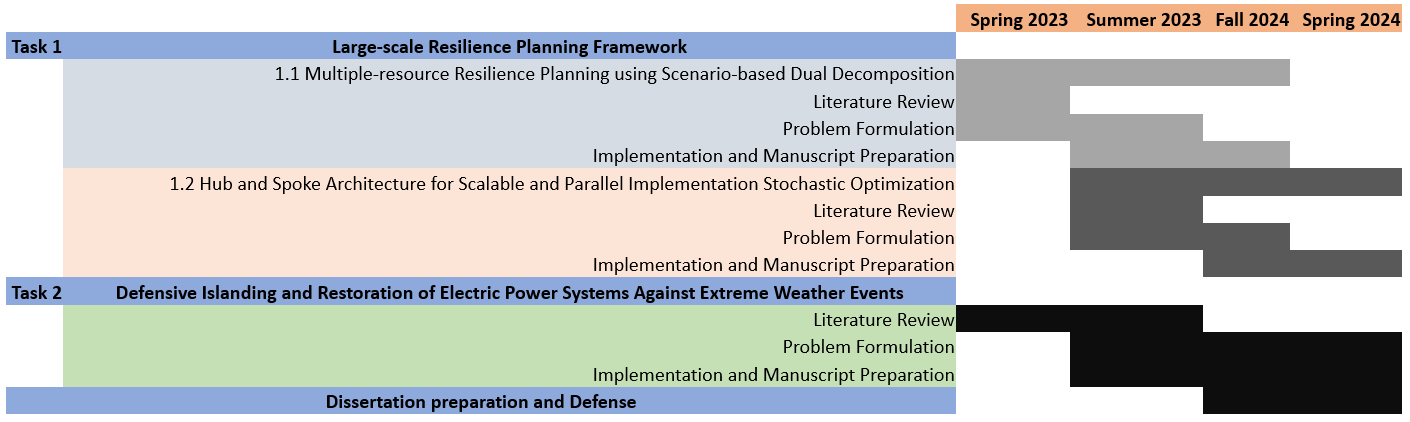
\includegraphics[width=0.99\textwidth]{images/timeline.eps}
  \vspace{-0.2 cm}
  \caption{\small Gantt chart showing execution plan for future works.}
\label{fig:time}
\end{figure}


\newpage
\section{Biography}
\small
Shiva Poudel received his B.E in Electrical Engineering from Insitute of Engineering, Pulchowk Campus, Kathmandu, Nepal in 2013, and M.S degree in Electrical Engineering from South Dakota State University, Brookings, SD in 2016. Currently, he is a graduate student in the School of
Electrical Engineering and Computer Science at Washington State University. His current research interests include distribution system modeling and analysis, restoration and resilience assessment.
\singlespacing
\subsection{Publications}
\small
\begin{enumerate}
    \item \textbf{S. Poudel} and A. Dubey, ``Critical Load Restoration using Distributed Energy Resources for Resilient Power Distribution System,'' in \textit{IEEE Transactions on Power Systems}, vol. 34, no. 1, pp. 52-63, Jan. 2019.
    \item \textbf{S. Poudel}, A. Dubey, A. Bose, and Kevin P. Schneider, ``Leveraging Distributed Generation Resources for Reliable and Resilient Power Distribution System,'' \textit{Submitted to IEEE Transactions on Sustainable Energy.}
    \item \textbf{S. Poudel}, A. Dubey, and A. Bose,  ``Risk-based Probabilistic Quantification of Power Distribution System Resilience,'' \textit{Submitted to IEEE Systems Journal.}
    
    \item A. Gandluru, \textbf{S. Poudel}, and A. Dubey,  ``Joint Estimation of Operational Topology and Outages for Unbalanced Power Distribution Systems,'' \textit{Submitted to IEEE Transactions on Power Systems.}
   \item A. Dubey and \textbf{S. Poudel}, “A robust approach to restoring critical loads in a resilient power distribution system,'', \textit{2017 IEEE Power \& Energy Society General Meeting,} Chicago, IL, 2017, pp. 1-5. \textcolor{red}{(``Presented at the best paper session'')}
    \item \textbf{S. Poudel} and A. Dubey, “A Graph-theoretic Framework for Electric Power Distribution System Service Restoration'', \textit{2018 IEEE Power \& Energy Society General Meeting}, Portland, OR, 2018, pp. 1-5.
    \item \textbf{S. Poudel}, A. Dubey, and M. Mukherjee, “Optimal Positioning of Mobile Emergency Resources for Resilient Restoration'', \textit{ 2018 North American Power Symposium (NAPS),} Fargo, ND, USA, 2018, pp. 1-6. \textcolor{red}{(``Received a second prize for the best paper award'')}
    \item M. Mukherjee, \textbf{S. Poudel}, A. Dubey, and A. Bose, “Distributed Generator Sizing for Joint Optimization of Resilience and Voltage Regulation'', \textit{ 2018 North American Power Symposium (NAPS),} Fargo, ND, USA, 2018, pp. 1-6.
    \item \textbf{S. Poudel}, A. Dubey, and A. Bose, “Probabilistic Quantification of Power Distribution System Operational Resilience'', \textit{Accepted to appear in IEEE Power \& Energy Society General Meeting}, 2019 Atlanta, GA.
    
\end{enumerate}    
\subsection{Course Work}


	\begin{table}[h]
	\small
	%\caption{Parameters of DERs for IEEE 906-bus test feeder}
	\begin{tabular}{l|l|l|l}
		\toprule
		\hline
		Course Number and Name & Semester taken& Instructor& Grade\\
		\hline
		EE 521 Power System Analysis& Fall 2016& Dr. Anjan Bose& A-\\
		EE 525 Power Electronics& Fall 2016& Dr. Mehardad Yazdanian& A-\\
		EE 521 Electromagnetics&  Fall2016& Dr. Patrick Pedrow& B+\\
		EE 511 Protection of Power Systems& Spring 2017& Dr. Saeed Lotfifard& A\\
		EE 523 Power System Stability and Control& Spring 2017& Dr. V. Venkatasubramanian& A-\\
		EE 538 Power System Economics& Fall 2017& Dr. Anurag Srivastava& A\\
		EE 432 RF Eng. for Telecommunications& Fall 2017& Dr. Ben Belzer& A\\
		EE 582 Power Quality& Spring 2018& Dr. Anamika Dubey& A\\
		\toprule
	\end{tabular}
	\vspace{-10 pt}
\end{table}


% BIBLIOGRAPHY %%%%%%%%%%%%%%%%%%%%%%%%%%%%%%%%%%%%%%%
\newpage

\bibliographystyle{ieeetr}
% \bibliography{bibliography}
% \fancyhead[R,OL]{bibliography}
\bibliography{bibliography}

\end{document}
